\begin{figure}[htbp]
\centering
\definecolor{sectionink}{RGB}{40,82,94}
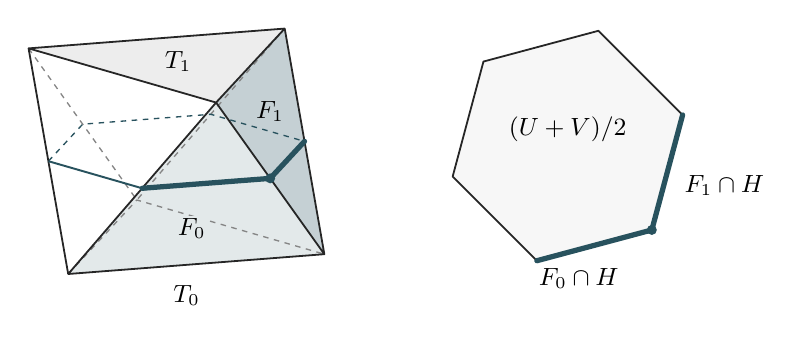
\begin{tikzpicture}[x=1.08cm,y=1.08cm,font=\small,line join=round,
    edge/.style={draw=black!85,line width=.65pt},
    hidden/.style={draw=black!48,line width=.48pt,dash pattern=on 2pt off 2pt},
    cut/.style={draw=sectionink,line width=.7pt},
    walk/.style={draw=sectionink,line width=1.9pt,line cap=round}]
  % View of a triangular antiprism with a horizontal middle section.
  \coordinate (u0) at (-1.273,-.368);
  \coordinate (u1) at (1.739,-.135);
  \coordinate (u2) at (-.466,.502);
  \coordinate (v0) at (.466,1.648);
  \coordinate (v1) at (1.273,2.518);
  \coordinate (v2) at (-1.739,2.285);
  \path (u0) -- coordinate[midway] (p1) (v0);
  \path (u1) -- coordinate[midway] (p2) (v0);
  \path (u1) -- coordinate[midway] (p3) (v1);
  \path (u2) -- coordinate[midway] (p4) (v1);
  \path (u2) -- coordinate[midway] (p5) (v2);
  \path (u0) -- coordinate[midway] (p6) (v2);
  \fill[black!7] (v0) -- (v1) -- (v2) -- cycle;
  \fill[sectionink!13] (u0) -- (u1) -- (v0) -- cycle;
  \fill[sectionink!27] (u1) -- (v1) -- (v0) -- cycle;
  \draw[hidden] (u0) -- (u2) -- (u1) (v2) -- (u2) -- (v1);
  \draw[hidden,sectionink] (p6) -- (p5) -- (p4) -- (p3);
  \draw[edge] (u0) -- (u1) -- (v1) -- (v2) -- cycle
    (u0) -- (v0) -- (u1) (v2) -- (v0) -- (v1);
  \draw[cut] (p6) -- (p1);
  \draw[walk] (p1) -- (p2) -- (p3);
  \fill[sectionink] (p2) circle (1.8pt);
  \node at (.02,2.13) {$T_1$};
  \node[fill=sectionink!13,inner sep=1pt] at (.18,.17) {$F_0$};
  \node[fill=sectionink!27,inner sep=1pt] at (1.10,1.54) {$F_1$};
  \node[below] at (.12,-.39) {$T_0$};
  % View of the same section from above, aligned left-to-right.
  \begin{scope}[shift={(4.60,1.14)}]
    \coordinate (q1) at (-.362,-1.352);
    \coordinate (q2) at (.990,-.990);
    \coordinate (q3) at (1.352,.362);
    \coordinate (q4) at (.362,1.352);
    \coordinate (q5) at (-.990,.990);
    \coordinate (q6) at (-1.352,-.362);
    \filldraw[fill=black!3,edge] (q1) -- (q2) -- (q3) -- (q4) --
      (q5) -- (q6) -- cycle;
    \draw[walk] (q1) -- (q2) -- (q3);
    \fill[sectionink] (q2) circle (1.8pt);
    \node at (0,.19) {$(U+V)/2$};
    \node[below] at (.13,-1.33) {$F_0\cap H$};
    \node[anchor=west] at (1.26,-.47) {$F_1\cap H$};
  \end{scope}
\end{tikzpicture}
\caption{The middle plane $H$ cuts a triangular antiprism in a hexagon.
The lateral facets $F_0,F_1$ meet along an edge with one endpoint
on each base. Its midpoint is the common vertex of the two highlighted
section edges. The three-step walk $T_0,F_0,F_1,T_1$ thus gives the
one-step walk $F_0\cap H,F_1\cap H$ in the section.}
\label{fig:prismatoid}
\end{figure}
